%%%%%%%%%%%%%%%%%%%%%%%%%%%%%%%%%%%%%%%%%%%%%%%%%%%%%%%%%%%%%%%%%%
\section{Herramientas software}
\label{sec:software}

\subsection{\acrshort{brite}}
\label{sec:brite}

\gls{brite} \cite{brite} se presenta como una plataforma dedicada a la generación de topologías de red. Fue desarrollada en la Universidad de Boston y se caracteriza por su gran flexibilidad, ya que enfoca su arquitectura en el concepto de modelo topológico. Es decir, soporta varios modelos diferentes y cada uno de ellos viene determinado por los parámetros de entrada que se definen. Es por ello que \gls{brite} sigue la siguiente secuencia de acciones para diseñar las topologías:

\vspace{3mm}

\begin{enumerate}
    \item Definición del posicionamiento de los nodos:
    \item Nivel de Interconexión de los nodos y configuración de enlaces:
    \item Asignación de atributos y características de la red y de los dispositivos: Se determina el delay y el ancho de banda de los enlaces.
    \item Especificación del formato de salida: Se indica un formato .brite para todas las topologías generadas.
\end{enumerate}

\vspace{3mm}

En la Sección \ref{sec:ejebrite} se definirán las acciones realizadas con esta herramienta en el caso de este \gls{tfm}. Por otro lado, con el motivo de facilitar el empleo de \gls{brite}, se incluirá una Sección dedicada al proceso de instalación, configuración y ejecución en el Anexo correspondiente a los manuales de usuario (ver Sección \ref{sec:manualbrite}). Se podrá acceder a más información desde el repositorio\footnote{https://github.com/NETSERV-UAH/BRITE} del equipo de investigación NetIS de la \gls{uah}.

\subsubsection{Definición de topologías}
\label{sec:param}

La herramienta \gls{brite} basa el proceso de creación de topologías en la definición de los siguientes parámetros de entrada en un fichero con formato .conf:

\begin{itemize}
    \item \textit{Name}: Modelo de la topología.
    \item \textit{N}: Número de nodos de la topología.  
    \item \textit{HS y LS}: Dimensiones del plano. Respectivamente, hacen referencia a la longitud total del plano cuadrado y al tamaño de los cuadros interiores.
    \item \textit{Node Placement}: Posicionamiento de los nodos. Se puede producir de forma totalmente aleatoria o creando zonas a lo largo del plano con mayor concentración de nodos. 
    \item \textit{Growth Type}: Método de introducción de los nodos en la topología. Se puede realizar este proceso de forma incremental (uno a uno) o de forma aleatoria (todos a la vez). 
    \item \textit{m}: Número de enlaces por nodo o número de nodos vecinos a los que se conectará un nuevo nodo al unirse a la red. \gls{brite} puede crear enlaces unidireccionales o bidireccionales y, respectivamente, la topología generada tendría un grado m o 2m.
    \item \textit{Alpha, Beta}: Parámetros específicos para topologías basadas en el modelo Waxman.
    \item \textit{BWDist, BWMin, BWMax}: Ancho de banda de los enlaces.
\end{itemize}

\subsubsection{Modelos de topologías}
\label{sec:modelostopos}

Como se ha introducido, con \gls{brite} se posibilita el uso de múltiples modelos para crear topologías. En la Figura \ref{fig:brite} se representan todos los que soporta la herramienta. No obstante, este \gls{tfm} se va a enfocar en la generación de topologías a nivel de router, como son los modelos Router Waxman y Router Barabasi-Albert. 

\vspace{3mm}

\begin{figure}[h!]
    \centering
    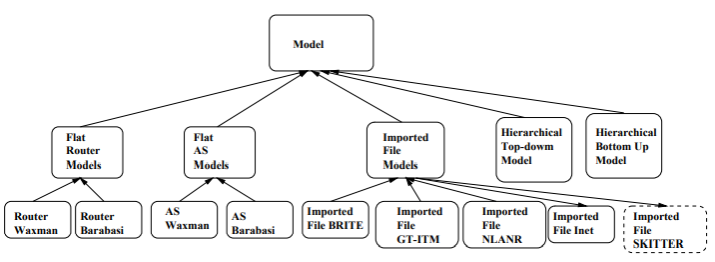
\includegraphics[width=1\textwidth]{img/teoria/brite.PNG}
    \caption{Modelos soportados por \acrshort{brite} \cite{brite}}
    \label{fig:brite}
\end{figure}

\vspace{3mm}

En el caso del Router Waxman, como su nombre indica, emplea un modelo de probabilidad Waxman para establecer la Interconexión de los nodos en la topología \cite{brite_zegura}:

\[P_{\text{Waxman}}(u,v) = \alpha \cdot e^{-\frac{d}{\beta \cdot L}}\]
    
    Donde:
\begin{itemize}
    \renewcommand{\labelitemi}{}
    \item \textit{P(u,v)} es la probabilidad en función de la distancia euclidiana entre un nodo \textit{u} y un nodo \textit{v} de la red.
    \item $\alpha$ es un parámetro específico del modelo que hace referencia a la densidad de enlaces y toma generalmente un valor igual a 0.2.
    \item $\beta$ es un parámetro específico del modelo que hace referencia al ratio enlaces largos/enlaces cortos en la topología y toma generalmente un valor igual a 0.15.
    \item \textit{L} es la máxima distancia entre dos nodos cualesquiera.
\end{itemize}

\vspace{3mm}

Por otro lado, el modelo Router Barabasi-Albert está basado en la generación de topologías con un incremento exponencial del número de nodos a lo largo del tiempo. Además, se permite una conexión preferencial, suponiendo que cuanto mayor grado de conectividad abarque un nodo, mayor será la probabilidad de que este añada nuevos enlaces. Por lo tanto, el plano de la topología comienza con un número de nodos inicial \textit{N0} y se van añadiendo los demás uno a uno. Cada uno de estos nuevos nodos se conectará a \textit{N} nodos ya añadidos a la topología con una probabilidad \cite{brite_zegura}:

\[P_{\text{Barabási-Albert}}(k_i) = \frac{k_i}{\sum_{j}^{}k_j}\]
    
    Donde:
\begin{itemize}
    \renewcommand{\labelitemi}{}
    \item \textit{P(k)} es la probabilidad de conexión del nodo \textit{i} con grado \textit{k}.
    \item $\sum_{j}^{}k_j$ es el sumatorio de los grados de todos los nodos de la topología.
\end{itemize}

\subsubsection{Automatización de la ejecución}
\label{sec:brite_eje}

A modo de facilitar la ejecución de la herramienta \gls{brite} se aporta en el repositorio el fichero de python \textit{generador\_brite.py}, dedicado a la automatización del proceso de creación de un fichero de configuración. Este recibirá los parámetros de entrada que caracterizarán a la topología a generar (ver Sección \ref{sec:param}) y escribirá el nuevo fichero.

\vspace{3mm}

También, se añade el fichero de python \textit{parser.py}, que se encargará de definir la función de transformación del archivo de salida proporcionado por \gls{brite} (en formato .brite) en dos nuevos ficheros: \textit{Nodos.txt} y \textit{Enlaces.txt}. Respectivamente, estos almacenarán las posiciones x e y de los nodos en el plano y la información sobre las distancias y los identificadores de los nodos que se interconectan con cada enlace. Este funcionamiento se muestra de forma gráfica en la Figura \ref{fig:parser}.

\vspace{3mm}

\begin{figure}[H]
    \centering
    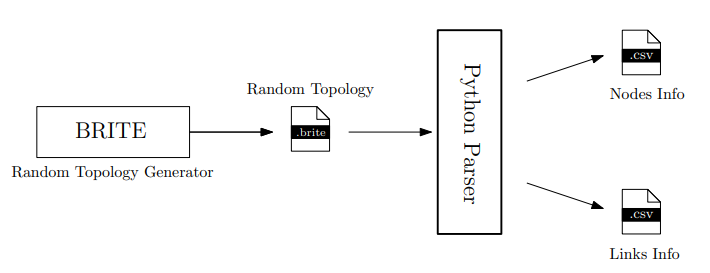
\includegraphics[width=0.7\textwidth]{img/teoria/parser.png}
    \caption{Esquema de funcionamiento de \acrshort{brite} y del \textit{parser} \cite{den2ne}}
    \label{fig:parser}
\end{figure}

\vspace{3mm}

Teniendo en cuenta los ficheros anteriores, se proporciona un script \textit{autogenerador.sh} donde se incluyen todas sus funcionalidades y se automatiza todo el proceso de ejecución de la herramienta. Este script sigue la siguiente secuencia de pasos:

\begin{enumerate}
    \item Define los valores de cada uno de los parámetros de entrada.
    \item Ejecuta el fichero de python \textit{generador\_brite.py} aplicando los parámetros definidos para el modelo Waxman y Barabasi.
    \item Genera 10 topologías diferentes para cada archivo de configuración a partir de 10 ficheros de semillas (\textit{seed\_files}) dados en el repositorio. Esto posibilita la generación de 10 topologías totalmente diferentes para cada escenario de red definido (a partir de unos mismos parámetros de entrada). 
    \item Se aplica un bucle en función del número de semilla:
    \begin{enumerate} 
        \item Crea el directorio para cada escenario y se ejecuta la heramienta \gls{brite} sobre cada uno.
        \item Se ejecuta \textit{parser.py} para obtener a la salida los ficheros \textit{Nodos.txt} y \textit{Enlaces.txt} de cada uno de los escenarios.   
    \end{enumerate} 
\end{enumerate}
